\documentclass[twoside]{book}

% Packages required by doxygen
\usepackage{calc}
\usepackage{doxygen}
\usepackage{graphicx}
\usepackage[utf8]{inputenc}
\usepackage{makeidx}
\usepackage{multicol}
\usepackage{multirow}
\usepackage{textcomp}
\usepackage[table]{xcolor}

% Font selection
\usepackage[T1]{fontenc}
\usepackage{mathptmx}
\usepackage[scaled=.90]{helvet}
\usepackage{courier}
\usepackage{amssymb}
\usepackage{sectsty}
\renewcommand{\familydefault}{\sfdefault}
\allsectionsfont{%
  \fontseries{bc}\selectfont%
  \color{darkgray}%
}
\renewcommand{\DoxyLabelFont}{%
  \fontseries{bc}\selectfont%
  \color{darkgray}%
}

% Page & text layout
\usepackage{geometry}
\geometry{%
  a4paper,%
  top=2.5cm,%
  bottom=2.5cm,%
  left=2.5cm,%
  right=2.5cm%
}
\tolerance=750
\hfuzz=15pt
\hbadness=750
\setlength{\emergencystretch}{15pt}
\setlength{\parindent}{0cm}
\setlength{\parskip}{0.2cm}
\makeatletter
\renewcommand{\paragraph}{%
  \@startsection{paragraph}{4}{0ex}{-1.0ex}{1.0ex}{%
    \normalfont\normalsize\bfseries\SS@parafont%
  }%
}
\renewcommand{\subparagraph}{%
  \@startsection{subparagraph}{5}{0ex}{-1.0ex}{1.0ex}{%
    \normalfont\normalsize\bfseries\SS@subparafont%
  }%
}
\makeatother

% Headers & footers
\usepackage{fancyhdr}
\pagestyle{fancyplain}
\fancyhead[LE]{\fancyplain{}{\bfseries\thepage}}
\fancyhead[CE]{\fancyplain{}{}}
\fancyhead[RE]{\fancyplain{}{\bfseries\leftmark}}
\fancyhead[LO]{\fancyplain{}{\bfseries\rightmark}}
\fancyhead[CO]{\fancyplain{}{}}
\fancyhead[RO]{\fancyplain{}{\bfseries\thepage}}
\fancyfoot[LE]{\fancyplain{}{}}
\fancyfoot[CE]{\fancyplain{}{}}
\fancyfoot[RE]{\fancyplain{}{\bfseries\scriptsize Generated on Mon Apr 11 2016 14\-:48\-:33 for User\-\_\-diagnostics by Doxygen }}
\fancyfoot[LO]{\fancyplain{}{\bfseries\scriptsize Generated on Mon Apr 11 2016 14\-:48\-:33 for User\-\_\-diagnostics by Doxygen }}
\fancyfoot[CO]{\fancyplain{}{}}
\fancyfoot[RO]{\fancyplain{}{}}
\renewcommand{\footrulewidth}{0.4pt}
\renewcommand{\chaptermark}[1]{%
  \markboth{#1}{}%
}
\renewcommand{\sectionmark}[1]{%
  \markright{\thesection\ #1}%
}

% Indices & bibliography
\usepackage{natbib}
\usepackage[titles]{tocloft}
\setcounter{tocdepth}{3}
\setcounter{secnumdepth}{5}
\makeindex

% Hyperlinks (required, but should be loaded last)
\usepackage{ifpdf}
\ifpdf
  \usepackage[pdftex,pagebackref=true]{hyperref}
\else
  \usepackage[ps2pdf,pagebackref=true]{hyperref}
\fi
\hypersetup{%
  colorlinks=true,%
  linkcolor=blue,%
  citecolor=blue,%
  unicode%
}

% Custom commands
\newcommand{\clearemptydoublepage}{%
  \newpage{\pagestyle{empty}\cleardoublepage}%
}


%===== C O N T E N T S =====

\begin{document}

% Titlepage & ToC
\hypersetup{pageanchor=false}
\pagenumbering{roman}
\begin{titlepage}
\vspace*{7cm}
\begin{center}%
{\Large User\-\_\-diagnostics }\\
\vspace*{1cm}
{\large Generated by Doxygen 1.8.6}\\
\vspace*{0.5cm}
{\small Mon Apr 11 2016 14:48:33}\\
\end{center}
\end{titlepage}
\clearemptydoublepage
\tableofcontents
\clearemptydoublepage
\pagenumbering{arabic}
\hypersetup{pageanchor=true}

%--- Begin generated contents ---
\chapter{Hierarchical Index}
\section{Class Hierarchy}
This inheritance list is sorted roughly, but not completely, alphabetically\-:\begin{DoxyCompactList}
\item \contentsline{section}{Admin\-Controller}{\pageref{class_admin_controller}}{}
\item \contentsline{section}{admin\-Model}{\pageref{classadmin_model}}{}
\item \contentsline{section}{Config}{\pageref{class_config}}{}
\item \contentsline{section}{Connect\-\_\-db}{\pageref{class_connect__db}}{}
\item \contentsline{section}{Connect\-\_\-\-S\-N\-M\-P}{\pageref{class_connect___s_n_m_p}}{}
\item \contentsline{section}{Controller}{\pageref{class_controller}}{}
\begin{DoxyCompactList}
\item \contentsline{section}{Index\-Controller}{\pageref{class_index_controller}}{}
\item \contentsline{section}{Node\-Controller}{\pageref{class_node_controller}}{}
\end{DoxyCompactList}
\item \contentsline{section}{Debugger}{\pageref{class_debugger}}{}
\item \contentsline{section}{error\-Model}{\pageref{classerror_model}}{}
\item \contentsline{section}{helper\-Model}{\pageref{classhelper_model}}{}
\item \contentsline{section}{history\-Model}{\pageref{classhistory_model}}{}
\item \contentsline{section}{Index\-Model}{\pageref{class_index_model}}{}
\item \contentsline{section}{Node\-Model}{\pageref{class_node_model}}{}
\item \contentsline{section}{pattern\-Model}{\pageref{classpattern_model}}{}
\item \contentsline{section}{Request}{\pageref{class_request}}{}
\item \contentsline{section}{Router}{\pageref{class_router}}{}
\item \contentsline{section}{Session}{\pageref{class_session}}{}
\end{DoxyCompactList}

\chapter{Data Structure Index}
\section{Data Structures}
Here are the data structures with brief descriptions\-:\begin{DoxyCompactList}
\item\contentsline{section}{\hyperlink{class_admin_controller}{Admin\-Controller} }{\pageref{class_admin_controller}}{}
\item\contentsline{section}{\hyperlink{classadmin_model}{admin\-Model} }{\pageref{classadmin_model}}{}
\item\contentsline{section}{\hyperlink{class_config}{Config} }{\pageref{class_config}}{}
\item\contentsline{section}{\hyperlink{class_connect__db}{Connect\-\_\-db} }{\pageref{class_connect__db}}{}
\item\contentsline{section}{\hyperlink{class_connect___s_n_m_p}{Connect\-\_\-\-S\-N\-M\-P} }{\pageref{class_connect___s_n_m_p}}{}
\item\contentsline{section}{\hyperlink{class_controller}{Controller} \\*Тестовый коментарий }{\pageref{class_controller}}{}
\item\contentsline{section}{\hyperlink{class_debugger}{Debugger} }{\pageref{class_debugger}}{}
\item\contentsline{section}{\hyperlink{classerror_model}{error\-Model} }{\pageref{classerror_model}}{}
\item\contentsline{section}{\hyperlink{classhelper_model}{helper\-Model} }{\pageref{classhelper_model}}{}
\item\contentsline{section}{\hyperlink{classhistory_model}{history\-Model} }{\pageref{classhistory_model}}{}
\item\contentsline{section}{\hyperlink{class_index_controller}{Index\-Controller} }{\pageref{class_index_controller}}{}
\item\contentsline{section}{\hyperlink{class_index_model}{Index\-Model} }{\pageref{class_index_model}}{}
\item\contentsline{section}{\hyperlink{class_node_controller}{Node\-Controller} }{\pageref{class_node_controller}}{}
\item\contentsline{section}{\hyperlink{class_node_model}{Node\-Model} }{\pageref{class_node_model}}{}
\item\contentsline{section}{\hyperlink{classpattern_model}{pattern\-Model} }{\pageref{classpattern_model}}{}
\item\contentsline{section}{\hyperlink{class_request}{Request} }{\pageref{class_request}}{}
\item\contentsline{section}{\hyperlink{class_router}{Router} }{\pageref{class_router}}{}
\item\contentsline{section}{\hyperlink{class_session}{Session} }{\pageref{class_session}}{}
\end{DoxyCompactList}

\chapter{Data Structure Documentation}
\hypertarget{class_admin_controller}{\section{Admin\-Controller Class Reference}
\label{class_admin_controller}\index{Admin\-Controller@{Admin\-Controller}}
}


The documentation for this class was generated from the following file\-:\begin{DoxyCompactItemize}
\item 
Controller/Admin\-Controller.\-php\end{DoxyCompactItemize}

\hypertarget{classadmin_model}{\section{Класс admin\-Model}
\label{classadmin_model}\index{admin\-Model@{admin\-Model}}
}
\subsection*{Открытые члены}
\begin{DoxyCompactItemize}
\item 
\hyperlink{classadmin_model_a1ccb28c3b18d4c5be588fee5fb49d03a}{\-\_\-\-\_\-construct} (\hyperlink{class_request}{Request} \$request, array \$pattern\-\_\-fields=null)
\item 
\hyperlink{classadmin_model_ae6200b0ddcbce08e8476b0704d4aa203}{is\-Valid\-Switch} ()
\item 
\hyperlink{classadmin_model_a8d26b64590b0f353c0ed9c2312473023}{is\-Valid\-Field\-Pattern} ()
\item 
\hyperlink{classadmin_model_a603807dbc8de64a7b6f690baa8d05b34}{check\-Insert\-Oid\-Data} ()
\item 
\hyperlink{classadmin_model_a3aae4149c7fed2165754b0f7b4da35a2}{insert\-Switch} ()
\item 
\hyperlink{classadmin_model_a53b7b03eb468bd378cdc5c0077e00d3d}{insert\-Pattern} ()
\item 
\hyperlink{classadmin_model_ad7be3392eeda63d39b61cbd6cdfcf046}{select\-Switch} ()
\item 
\hyperlink{classadmin_model_a94c19717b6cc43f904d04e88dac324d5}{select\-Switch\-By\-Name\-Firmware} ()
\item 
\hyperlink{classadmin_model_a886c60eae2d65d7e030ce86f8b7d1641}{select\-Switch\-By\-I\-D} (\$id\-\_\-switch)
\item 
\hyperlink{classadmin_model_aca44164fba29f506cb9ec0ea706072b3}{select\-Pattern\-By\-I\-D} (\$id\-\_\-pattern)
\item 
\hyperlink{classadmin_model_af26cb48d302aa8379acbb4f638b4e26f}{edit\-Switch} (\$id\-\_\-switch)
\item 
\hyperlink{classadmin_model_a898e504409c304470890e25a5673295f}{edit\-Pattern} (\$id\-\_\-pattern)
\item 
\hyperlink{classadmin_model_a02146a7ee4437df5d8526bdcddd72998}{delete\-Switch} (\$id\-\_\-switch)
\item 
\hyperlink{classadmin_model_a1d302d77f014aeaf0b313ab439504a33}{delete\-Pattern} (\$id\-\_\-pattern)
\item 
\hyperlink{classadmin_model_a573d43eeee3b961db22cc05cbdd5d26a}{get\-Pattern\-Fields\-Value} ()
\end{DoxyCompactItemize}
\subsection*{Поля данных}
\begin{DoxyCompactItemize}
\item 
\hyperlink{classadmin_model_ac4551d8a2764c22fc62f61d13b12670f}{\$switch\-\_\-name}
\item 
\hyperlink{classadmin_model_a2b1ea6f804c1caa0c3e824412fe37b16}{\$switch\-\_\-manufacturer}
\item 
\hyperlink{classadmin_model_aaba9e06ee8c7745e9ffc30dbdb001f0a}{\$switch\-\_\-firmware}
\item 
\hyperlink{classadmin_model_a1f184554798f3454ffece10936bd9990}{\$switch\-\_\-simple\-\_\-ports}
\item 
\hyperlink{classadmin_model_aa33faaec4d5d8fe44e40333da0d4734f}{\$switch\-\_\-gig\-\_\-ports}
\item 
\hyperlink{classadmin_model_af374d5f9d4e5b9dca9e10c4053ddbd3b}{\$pattern\-\_\-id}
\item 
\hyperlink{classadmin_model_a8543536fb1742f29ceee9f3827119d0c}{\$pattern\-\_\-fields\-\_\-value} = array()
\item 
\hyperlink{classadmin_model_aeaf349782ab66700c60fa2a0f49853dd}{\$pattern\-\_\-field\-\_\-check} = array()
\end{DoxyCompactItemize}


\subsection{Подробное описание}


См. определение в файле admin\-Model.\-php строка 4



\subsection{Конструктор(ы)}
\hypertarget{classadmin_model_a1ccb28c3b18d4c5be588fee5fb49d03a}{\index{admin\-Model@{admin\-Model}!\-\_\-\-\_\-construct@{\-\_\-\-\_\-construct}}
\index{\-\_\-\-\_\-construct@{\-\_\-\-\_\-construct}!adminModel@{admin\-Model}}
\subsubsection[{\-\_\-\-\_\-construct}]{\setlength{\rightskip}{0pt plus 5cm}\-\_\-\-\_\-construct (
\begin{DoxyParamCaption}
\item[{{\bf Request}}]{\$request, }
\item[{array}]{\$pattern\-\_\-fields = {\ttfamily null}}
\end{DoxyParamCaption}
)}}\label{classadmin_model_a1ccb28c3b18d4c5be588fee5fb49d03a}


См. определение в файле admin\-Model.\-php строка 16



\subsection{Методы}
\hypertarget{classadmin_model_a603807dbc8de64a7b6f690baa8d05b34}{\index{admin\-Model@{admin\-Model}!check\-Insert\-Oid\-Data@{check\-Insert\-Oid\-Data}}
\index{check\-Insert\-Oid\-Data@{check\-Insert\-Oid\-Data}!adminModel@{admin\-Model}}
\subsubsection[{check\-Insert\-Oid\-Data}]{\setlength{\rightskip}{0pt plus 5cm}check\-Insert\-Oid\-Data (
\begin{DoxyParamCaption}
{}
\end{DoxyParamCaption}
)}}\label{classadmin_model_a603807dbc8de64a7b6f690baa8d05b34}


См. определение в файле admin\-Model.\-php строка 75

\hypertarget{classadmin_model_a1d302d77f014aeaf0b313ab439504a33}{\index{admin\-Model@{admin\-Model}!delete\-Pattern@{delete\-Pattern}}
\index{delete\-Pattern@{delete\-Pattern}!adminModel@{admin\-Model}}
\subsubsection[{delete\-Pattern}]{\setlength{\rightskip}{0pt plus 5cm}delete\-Pattern (
\begin{DoxyParamCaption}
\item[{}]{\$id\-\_\-pattern}
\end{DoxyParamCaption}
)}}\label{classadmin_model_a1d302d77f014aeaf0b313ab439504a33}


См. определение в файле admin\-Model.\-php строка 237

\hypertarget{classadmin_model_a02146a7ee4437df5d8526bdcddd72998}{\index{admin\-Model@{admin\-Model}!delete\-Switch@{delete\-Switch}}
\index{delete\-Switch@{delete\-Switch}!adminModel@{admin\-Model}}
\subsubsection[{delete\-Switch}]{\setlength{\rightskip}{0pt plus 5cm}delete\-Switch (
\begin{DoxyParamCaption}
\item[{}]{\$id\-\_\-switch}
\end{DoxyParamCaption}
)}}\label{classadmin_model_a02146a7ee4437df5d8526bdcddd72998}


См. определение в файле admin\-Model.\-php строка 225

\hypertarget{classadmin_model_a898e504409c304470890e25a5673295f}{\index{admin\-Model@{admin\-Model}!edit\-Pattern@{edit\-Pattern}}
\index{edit\-Pattern@{edit\-Pattern}!adminModel@{admin\-Model}}
\subsubsection[{edit\-Pattern}]{\setlength{\rightskip}{0pt plus 5cm}edit\-Pattern (
\begin{DoxyParamCaption}
\item[{}]{\$id\-\_\-pattern}
\end{DoxyParamCaption}
)}}\label{classadmin_model_a898e504409c304470890e25a5673295f}


См. определение в файле admin\-Model.\-php строка 199

\hypertarget{classadmin_model_af26cb48d302aa8379acbb4f638b4e26f}{\index{admin\-Model@{admin\-Model}!edit\-Switch@{edit\-Switch}}
\index{edit\-Switch@{edit\-Switch}!adminModel@{admin\-Model}}
\subsubsection[{edit\-Switch}]{\setlength{\rightskip}{0pt plus 5cm}edit\-Switch (
\begin{DoxyParamCaption}
\item[{}]{\$id\-\_\-switch}
\end{DoxyParamCaption}
)}}\label{classadmin_model_af26cb48d302aa8379acbb4f638b4e26f}


См. определение в файле admin\-Model.\-php строка 182

\hypertarget{classadmin_model_a573d43eeee3b961db22cc05cbdd5d26a}{\index{admin\-Model@{admin\-Model}!get\-Pattern\-Fields\-Value@{get\-Pattern\-Fields\-Value}}
\index{get\-Pattern\-Fields\-Value@{get\-Pattern\-Fields\-Value}!adminModel@{admin\-Model}}
\subsubsection[{get\-Pattern\-Fields\-Value}]{\setlength{\rightskip}{0pt plus 5cm}get\-Pattern\-Fields\-Value (
\begin{DoxyParamCaption}
{}
\end{DoxyParamCaption}
)}}\label{classadmin_model_a573d43eeee3b961db22cc05cbdd5d26a}
\begin{DoxyReturn}{Возвращает}
array 
\end{DoxyReturn}


См. определение в файле admin\-Model.\-php строка 252

\hypertarget{classadmin_model_a53b7b03eb468bd378cdc5c0077e00d3d}{\index{admin\-Model@{admin\-Model}!insert\-Pattern@{insert\-Pattern}}
\index{insert\-Pattern@{insert\-Pattern}!adminModel@{admin\-Model}}
\subsubsection[{insert\-Pattern}]{\setlength{\rightskip}{0pt plus 5cm}insert\-Pattern (
\begin{DoxyParamCaption}
{}
\end{DoxyParamCaption}
)}}\label{classadmin_model_a53b7b03eb468bd378cdc5c0077e00d3d}


См. определение в файле admin\-Model.\-php строка 113

\hypertarget{classadmin_model_a3aae4149c7fed2165754b0f7b4da35a2}{\index{admin\-Model@{admin\-Model}!insert\-Switch@{insert\-Switch}}
\index{insert\-Switch@{insert\-Switch}!adminModel@{admin\-Model}}
\subsubsection[{insert\-Switch}]{\setlength{\rightskip}{0pt plus 5cm}insert\-Switch (
\begin{DoxyParamCaption}
{}
\end{DoxyParamCaption}
)}}\label{classadmin_model_a3aae4149c7fed2165754b0f7b4da35a2}


См. определение в файле admin\-Model.\-php строка 96

\hypertarget{classadmin_model_a8d26b64590b0f353c0ed9c2312473023}{\index{admin\-Model@{admin\-Model}!is\-Valid\-Field\-Pattern@{is\-Valid\-Field\-Pattern}}
\index{is\-Valid\-Field\-Pattern@{is\-Valid\-Field\-Pattern}!adminModel@{admin\-Model}}
\subsubsection[{is\-Valid\-Field\-Pattern}]{\setlength{\rightskip}{0pt plus 5cm}is\-Valid\-Field\-Pattern (
\begin{DoxyParamCaption}
{}
\end{DoxyParamCaption}
)}}\label{classadmin_model_a8d26b64590b0f353c0ed9c2312473023}


См. определение в файле admin\-Model.\-php строка 62

\hypertarget{classadmin_model_ae6200b0ddcbce08e8476b0704d4aa203}{\index{admin\-Model@{admin\-Model}!is\-Valid\-Switch@{is\-Valid\-Switch}}
\index{is\-Valid\-Switch@{is\-Valid\-Switch}!adminModel@{admin\-Model}}
\subsubsection[{is\-Valid\-Switch}]{\setlength{\rightskip}{0pt plus 5cm}is\-Valid\-Switch (
\begin{DoxyParamCaption}
{}
\end{DoxyParamCaption}
)}}\label{classadmin_model_ae6200b0ddcbce08e8476b0704d4aa203}


См. определение в файле admin\-Model.\-php строка 44

\hypertarget{classadmin_model_aca44164fba29f506cb9ec0ea706072b3}{\index{admin\-Model@{admin\-Model}!select\-Pattern\-By\-I\-D@{select\-Pattern\-By\-I\-D}}
\index{select\-Pattern\-By\-I\-D@{select\-Pattern\-By\-I\-D}!adminModel@{admin\-Model}}
\subsubsection[{select\-Pattern\-By\-I\-D}]{\setlength{\rightskip}{0pt plus 5cm}select\-Pattern\-By\-I\-D (
\begin{DoxyParamCaption}
\item[{}]{\$id\-\_\-pattern}
\end{DoxyParamCaption}
)}}\label{classadmin_model_aca44164fba29f506cb9ec0ea706072b3}


См. определение в файле admin\-Model.\-php строка 170

\hypertarget{classadmin_model_ad7be3392eeda63d39b61cbd6cdfcf046}{\index{admin\-Model@{admin\-Model}!select\-Switch@{select\-Switch}}
\index{select\-Switch@{select\-Switch}!adminModel@{admin\-Model}}
\subsubsection[{select\-Switch}]{\setlength{\rightskip}{0pt plus 5cm}select\-Switch (
\begin{DoxyParamCaption}
{}
\end{DoxyParamCaption}
)}}\label{classadmin_model_ad7be3392eeda63d39b61cbd6cdfcf046}


См. определение в файле admin\-Model.\-php строка 134

\hypertarget{classadmin_model_a886c60eae2d65d7e030ce86f8b7d1641}{\index{admin\-Model@{admin\-Model}!select\-Switch\-By\-I\-D@{select\-Switch\-By\-I\-D}}
\index{select\-Switch\-By\-I\-D@{select\-Switch\-By\-I\-D}!adminModel@{admin\-Model}}
\subsubsection[{select\-Switch\-By\-I\-D}]{\setlength{\rightskip}{0pt plus 5cm}select\-Switch\-By\-I\-D (
\begin{DoxyParamCaption}
\item[{}]{\$id\-\_\-switch}
\end{DoxyParamCaption}
)}}\label{classadmin_model_a886c60eae2d65d7e030ce86f8b7d1641}


См. определение в файле admin\-Model.\-php строка 158

\hypertarget{classadmin_model_a94c19717b6cc43f904d04e88dac324d5}{\index{admin\-Model@{admin\-Model}!select\-Switch\-By\-Name\-Firmware@{select\-Switch\-By\-Name\-Firmware}}
\index{select\-Switch\-By\-Name\-Firmware@{select\-Switch\-By\-Name\-Firmware}!adminModel@{admin\-Model}}
\subsubsection[{select\-Switch\-By\-Name\-Firmware}]{\setlength{\rightskip}{0pt plus 5cm}select\-Switch\-By\-Name\-Firmware (
\begin{DoxyParamCaption}
{}
\end{DoxyParamCaption}
)}}\label{classadmin_model_a94c19717b6cc43f904d04e88dac324d5}


См. определение в файле admin\-Model.\-php строка 145



\subsection{Поля}
\hypertarget{classadmin_model_aeaf349782ab66700c60fa2a0f49853dd}{\index{admin\-Model@{admin\-Model}!\$pattern\-\_\-field\-\_\-check@{\$pattern\-\_\-field\-\_\-check}}
\index{\$pattern\-\_\-field\-\_\-check@{\$pattern\-\_\-field\-\_\-check}!adminModel@{admin\-Model}}
\subsubsection[{\$pattern\-\_\-field\-\_\-check}]{\setlength{\rightskip}{0pt plus 5cm}\$pattern\-\_\-field\-\_\-check = array()}}\label{classadmin_model_aeaf349782ab66700c60fa2a0f49853dd}


См. определение в файле admin\-Model.\-php строка 14

\hypertarget{classadmin_model_a8543536fb1742f29ceee9f3827119d0c}{\index{admin\-Model@{admin\-Model}!\$pattern\-\_\-fields\-\_\-value@{\$pattern\-\_\-fields\-\_\-value}}
\index{\$pattern\-\_\-fields\-\_\-value@{\$pattern\-\_\-fields\-\_\-value}!adminModel@{admin\-Model}}
\subsubsection[{\$pattern\-\_\-fields\-\_\-value}]{\setlength{\rightskip}{0pt plus 5cm}\$pattern\-\_\-fields\-\_\-value = array()}}\label{classadmin_model_a8543536fb1742f29ceee9f3827119d0c}


См. определение в файле admin\-Model.\-php строка 13

\hypertarget{classadmin_model_af374d5f9d4e5b9dca9e10c4053ddbd3b}{\index{admin\-Model@{admin\-Model}!\$pattern\-\_\-id@{\$pattern\-\_\-id}}
\index{\$pattern\-\_\-id@{\$pattern\-\_\-id}!adminModel@{admin\-Model}}
\subsubsection[{\$pattern\-\_\-id}]{\setlength{\rightskip}{0pt plus 5cm}\$pattern\-\_\-id}}\label{classadmin_model_af374d5f9d4e5b9dca9e10c4053ddbd3b}


См. определение в файле admin\-Model.\-php строка 12

\hypertarget{classadmin_model_aaba9e06ee8c7745e9ffc30dbdb001f0a}{\index{admin\-Model@{admin\-Model}!\$switch\-\_\-firmware@{\$switch\-\_\-firmware}}
\index{\$switch\-\_\-firmware@{\$switch\-\_\-firmware}!adminModel@{admin\-Model}}
\subsubsection[{\$switch\-\_\-firmware}]{\setlength{\rightskip}{0pt plus 5cm}\$switch\-\_\-firmware}}\label{classadmin_model_aaba9e06ee8c7745e9ffc30dbdb001f0a}


См. определение в файле admin\-Model.\-php строка 9

\hypertarget{classadmin_model_aa33faaec4d5d8fe44e40333da0d4734f}{\index{admin\-Model@{admin\-Model}!\$switch\-\_\-gig\-\_\-ports@{\$switch\-\_\-gig\-\_\-ports}}
\index{\$switch\-\_\-gig\-\_\-ports@{\$switch\-\_\-gig\-\_\-ports}!adminModel@{admin\-Model}}
\subsubsection[{\$switch\-\_\-gig\-\_\-ports}]{\setlength{\rightskip}{0pt plus 5cm}\$switch\-\_\-gig\-\_\-ports}}\label{classadmin_model_aa33faaec4d5d8fe44e40333da0d4734f}


См. определение в файле admin\-Model.\-php строка 11

\hypertarget{classadmin_model_a2b1ea6f804c1caa0c3e824412fe37b16}{\index{admin\-Model@{admin\-Model}!\$switch\-\_\-manufacturer@{\$switch\-\_\-manufacturer}}
\index{\$switch\-\_\-manufacturer@{\$switch\-\_\-manufacturer}!adminModel@{admin\-Model}}
\subsubsection[{\$switch\-\_\-manufacturer}]{\setlength{\rightskip}{0pt plus 5cm}\$switch\-\_\-manufacturer}}\label{classadmin_model_a2b1ea6f804c1caa0c3e824412fe37b16}


См. определение в файле admin\-Model.\-php строка 8

\hypertarget{classadmin_model_ac4551d8a2764c22fc62f61d13b12670f}{\index{admin\-Model@{admin\-Model}!\$switch\-\_\-name@{\$switch\-\_\-name}}
\index{\$switch\-\_\-name@{\$switch\-\_\-name}!adminModel@{admin\-Model}}
\subsubsection[{\$switch\-\_\-name}]{\setlength{\rightskip}{0pt plus 5cm}\$switch\-\_\-name}}\label{classadmin_model_ac4551d8a2764c22fc62f61d13b12670f}


См. определение в файле admin\-Model.\-php строка 7

\hypertarget{classadmin_model_a1f184554798f3454ffece10936bd9990}{\index{admin\-Model@{admin\-Model}!\$switch\-\_\-simple\-\_\-ports@{\$switch\-\_\-simple\-\_\-ports}}
\index{\$switch\-\_\-simple\-\_\-ports@{\$switch\-\_\-simple\-\_\-ports}!adminModel@{admin\-Model}}
\subsubsection[{\$switch\-\_\-simple\-\_\-ports}]{\setlength{\rightskip}{0pt plus 5cm}\$switch\-\_\-simple\-\_\-ports}}\label{classadmin_model_a1f184554798f3454ffece10936bd9990}


См. определение в файле admin\-Model.\-php строка 10



Объявления и описания членов класса находятся в файле\-:\begin{DoxyCompactItemize}
\item 
/home/artem/public\-\_\-html/test01/\-Model/\hyperlink{admin_model_8php}{admin\-Model.\-php}\end{DoxyCompactItemize}

\hypertarget{class_config}{\section{Config Class Reference}
\label{class_config}\index{Config@{Config}}
}
\subsection*{Static Public Member Functions}
\begin{DoxyCompactItemize}
\item 
\hypertarget{class_config_a15e2679f2a8f6fa4d60757f4d65413ac}{static {\bfseries get} (\$key)}\label{class_config_a15e2679f2a8f6fa4d60757f4d65413ac}

\item 
\hypertarget{class_config_aa485369b2925858d92e468d405bd0798}{static {\bfseries set} (\$key, \$value)}\label{class_config_aa485369b2925858d92e468d405bd0798}

\end{DoxyCompactItemize}
\subsection*{Static Protected Attributes}
\begin{DoxyCompactItemize}
\item 
\hypertarget{class_config_ac7c3353107070daa85f641882931b358}{static {\bfseries \$settings} = array()}\label{class_config_ac7c3353107070daa85f641882931b358}

\end{DoxyCompactItemize}


The documentation for this class was generated from the following file\-:\begin{DoxyCompactItemize}
\item 
Library/Config.\-php\end{DoxyCompactItemize}

\hypertarget{class_connect__db}{\section{Connect\-\_\-db Class Reference}
\label{class_connect__db}\index{Connect\-\_\-db@{Connect\-\_\-db}}
}
\subsection*{Public Member Functions}
\begin{DoxyCompactItemize}
\item 
\hypertarget{class_connect__db_a064a8657e9547cedc4e1590fb8c7747f}{{\bfseries get\-Date} (\$sql, array \$placeholders=array())}\label{class_connect__db_a064a8657e9547cedc4e1590fb8c7747f}

\item 
\hypertarget{class_connect__db_af708fa20ff0c04a5a9bd8badd63e632c}{{\bfseries get\-P\-D\-O} ()}\label{class_connect__db_af708fa20ff0c04a5a9bd8badd63e632c}

\end{DoxyCompactItemize}
\subsection*{Static Public Member Functions}
\begin{DoxyCompactItemize}
\item 
\hypertarget{class_connect__db_ab6bc68b89cd8ca077dd8ab2c5a357f06}{static {\bfseries get\-Connection} (\$db\-\_\-number=1)}\label{class_connect__db_ab6bc68b89cd8ca077dd8ab2c5a357f06}

\end{DoxyCompactItemize}


The documentation for this class was generated from the following file\-:\begin{DoxyCompactItemize}
\item 
Library/Connect\-\_\-db.\-php\end{DoxyCompactItemize}

\hypertarget{class_connect___s_n_m_p}{\section{Connect\-\_\-\-S\-N\-M\-P Class Reference}
\label{class_connect___s_n_m_p}\index{Connect\-\_\-\-S\-N\-M\-P@{Connect\-\_\-\-S\-N\-M\-P}}
}
\subsection*{Public Member Functions}
\begin{DoxyCompactItemize}
\item 
\hypertarget{class_connect___s_n_m_p_a8a4beac9f8314f8e4f86f29b4cf619a0}{{\bfseries \-\_\-\-\_\-construct} (\$switch\-\_\-ip, \$wr\-\_\-rd= 'r')}\label{class_connect___s_n_m_p_a8a4beac9f8314f8e4f86f29b4cf619a0}

\item 
\hypertarget{class_connect___s_n_m_p_a2266e0810688c5e97603e08be2733771}{{\bfseries close\-\_\-session} ()}\label{class_connect___s_n_m_p_a2266e0810688c5e97603e08be2733771}

\item 
\hypertarget{class_connect___s_n_m_p_ad6dcf9d79ad7d6839e1639c3d6f1ce47}{{\bfseries get\-By\-Key} (\$key)}\label{class_connect___s_n_m_p_ad6dcf9d79ad7d6839e1639c3d6f1ce47}

\item 
\hypertarget{class_connect___s_n_m_p_a7d9b0650197ccf543efa794508f7fbd6}{{\bfseries set\-Data} (\$object\-\_\-id, \$type, \$value)}\label{class_connect___s_n_m_p_a7d9b0650197ccf543efa794508f7fbd6}

\item 
\hypertarget{class_connect___s_n_m_p_a0cf9c2e32cb02151e4d117af3ec13b39}{{\bfseries walk\-By\-Key} (\$key)}\label{class_connect___s_n_m_p_a0cf9c2e32cb02151e4d117af3ec13b39}

\item 
\hyperlink{class_connect___s_n_m_p_a91a834f81bf2db67f0523d92666db887}{get\-Snmp\-Session} ()
\end{DoxyCompactItemize}


\subsection{Member Function Documentation}
\hypertarget{class_connect___s_n_m_p_a91a834f81bf2db67f0523d92666db887}{\index{Connect\-\_\-\-S\-N\-M\-P@{Connect\-\_\-\-S\-N\-M\-P}!get\-Snmp\-Session@{get\-Snmp\-Session}}
\index{get\-Snmp\-Session@{get\-Snmp\-Session}!Connect_SNMP@{Connect\-\_\-\-S\-N\-M\-P}}
\subsubsection[{get\-Snmp\-Session}]{\setlength{\rightskip}{0pt plus 5cm}get\-Snmp\-Session (
\begin{DoxyParamCaption}
{}
\end{DoxyParamCaption}
)}}\label{class_connect___s_n_m_p_a91a834f81bf2db67f0523d92666db887}
\begin{DoxyReturn}{Returns}
S\-N\-M\-P 
\end{DoxyReturn}


The documentation for this class was generated from the following file\-:\begin{DoxyCompactItemize}
\item 
Library/Connect\-\_\-\-S\-N\-M\-P.\-php\end{DoxyCompactItemize}

\hypertarget{class_controller}{\section{Класс Controller}
\label{class_controller}\index{Controller@{Controller}}
}


Class \hyperlink{class_controller}{Controller}.  


Граф наследования\-:Controller\-:\begin{figure}[H]
\begin{center}
\leavevmode
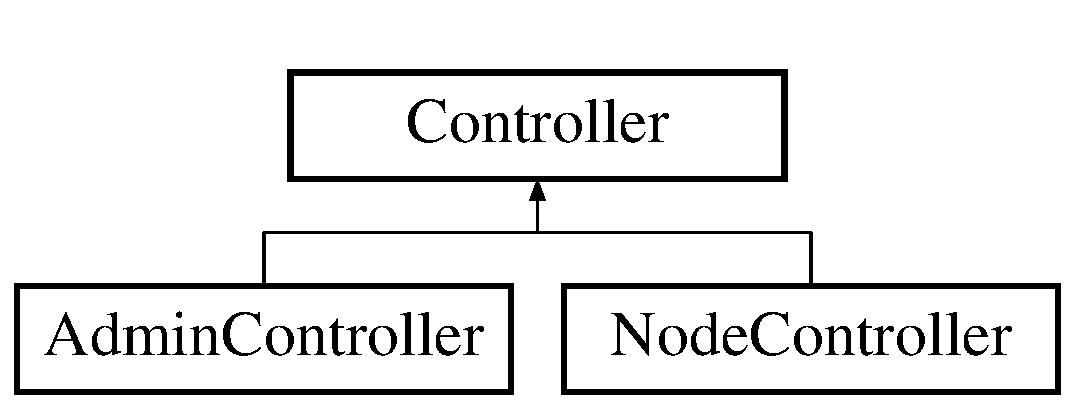
\includegraphics[height=2.000000cm]{class_controller}
\end{center}
\end{figure}
\subsection*{Открытые статические члены}
\begin{DoxyCompactItemize}
\item 
static \hyperlink{class_controller_a4c9227317bc5a987371b5eb4407f75e1}{redirect} (\$url)
\end{DoxyCompactItemize}
\subsection*{Защищенные члены}
\begin{DoxyCompactItemize}
\item 
\hyperlink{class_controller_a87cbafbc85f49bc8864557e1ffe0c143}{render} (array \$args=array(), \$tpl=null)
\begin{DoxyCompactList}\small\item\em Рендеринг обычных страниц \end{DoxyCompactList}\item 
\hyperlink{class_controller_a97e0e46d82368469d174861ca29f2001}{render\-\_\-admin} (array \$args=array(), \$tpl=null)
\end{DoxyCompactItemize}


\subsection{Подробное описание}
Class \hyperlink{class_controller}{Controller}. 

Отвечает за рендеринг, редиректы 

См. определение в файле Controller.\-php строка 9



\subsection{Методы}
\hypertarget{class_controller_a4c9227317bc5a987371b5eb4407f75e1}{\index{Controller@{Controller}!redirect@{redirect}}
\index{redirect@{redirect}!Controller@{Controller}}
\subsubsection[{redirect}]{\setlength{\rightskip}{0pt plus 5cm}static redirect (
\begin{DoxyParamCaption}
\item[{}]{\$url}
\end{DoxyParamCaption}
)\hspace{0.3cm}{\ttfamily [static]}}}\label{class_controller_a4c9227317bc5a987371b5eb4407f75e1}


См. определение в файле Controller.\-php строка 97

\hypertarget{class_controller_a87cbafbc85f49bc8864557e1ffe0c143}{\index{Controller@{Controller}!render@{render}}
\index{render@{render}!Controller@{Controller}}
\subsubsection[{render}]{\setlength{\rightskip}{0pt plus 5cm}render (
\begin{DoxyParamCaption}
\item[{array}]{\$args = {\ttfamily array()}, }
\item[{}]{\$tpl = {\ttfamily null}}
\end{DoxyParamCaption}
)\hspace{0.3cm}{\ttfamily [protected]}}}\label{class_controller_a87cbafbc85f49bc8864557e1ffe0c143}


Рендеринг обычных страниц 


\begin{DoxyParams}{Аргументы}
{\em \$arg} & Массив переменных передаваемые в шаблон для отображения \\
\hline
{\em \$tpl} & имя файла шаблона по умолчанию = null если оно отличается от имени дейстия (Action)\\
\hline
\end{DoxyParams}
Переменные из массива \$args используются в файлах шаблонов для вывода необходимого контента.\-В буфер обмена записывается сначала результат рендеринга необходимого шаблона, результат передается переменной \$content. После этого из буфера обмена выгружатеся вся страница в виде основного шаблона \hyperlink{layout_8phtml}{layout.\-phtml} или \hyperlink{layout__billing_8phtml}{layout\-\_\-billing.\-phtml} в котором встроенна переменная \$content, содержащая основной контент. Используются различные лайауты \hyperlink{layout_8phtml}{layout.\-phtml} или \hyperlink{layout__billing_8phtml}{layout\-\_\-billing.\-phtml} в зависимости от запроса страници -\/ если запрос произошел из биллинга (еслиь get параметр 'bl') -\/layout\-\_\-billing.\-phtml, если запрос из самого приложения обычный лайаут.

\begin{DoxyReturn}{Возвращает}
ob\-\_\-get\-\_\-clean() Отрендеренную страницу из буфера обмена 
\end{DoxyReturn}


См. определение в файле Controller.\-php строка 60

\hypertarget{class_controller_a97e0e46d82368469d174861ca29f2001}{\index{Controller@{Controller}!render\-\_\-admin@{render\-\_\-admin}}
\index{render\-\_\-admin@{render\-\_\-admin}!Controller@{Controller}}
\subsubsection[{render\-\_\-admin}]{\setlength{\rightskip}{0pt plus 5cm}render\-\_\-admin (
\begin{DoxyParamCaption}
\item[{array}]{\$args = {\ttfamily array()}, }
\item[{}]{\$tpl = {\ttfamily null}}
\end{DoxyParamCaption}
)\hspace{0.3cm}{\ttfamily [protected]}}}\label{class_controller_a97e0e46d82368469d174861ca29f2001}


См. определение в файле Controller.\-php строка 80



Объявления и описания членов класса находятся в файле\-:\begin{DoxyCompactItemize}
\item 
/home/artem/public\-\_\-html/test01/\-Library/\hyperlink{_controller_8php}{Controller.\-php}\end{DoxyCompactItemize}

\hypertarget{class_debugger}{\section{Debugger Class Reference}
\label{class_debugger}\index{Debugger@{Debugger}}
}
\subsection*{Static Public Member Functions}
\begin{DoxyCompactItemize}
\item 
\hypertarget{class_debugger_aabc92ba8fe7187ce953d8edbb3175e78}{static {\bfseries Print\-R} (\$item)}\label{class_debugger_aabc92ba8fe7187ce953d8edbb3175e78}

\item 
\hypertarget{class_debugger_a54d5010505863da589f9355a898c4116}{static {\bfseries Var\-Damp} (\$item)}\label{class_debugger_a54d5010505863da589f9355a898c4116}

\end{DoxyCompactItemize}


The documentation for this class was generated from the following file\-:\begin{DoxyCompactItemize}
\item 
Library/Debugger.\-php\end{DoxyCompactItemize}

\hypertarget{classerror_model}{\section{Класс error\-Model}
\label{classerror_model}\index{error\-Model@{error\-Model}}
}
\subsection*{Открытые члены}
\begin{DoxyCompactItemize}
\item 
\hyperlink{classerror_model_a4ed8d21ed582ab26d9d813e9f44251d7}{\-\_\-\-\_\-construct} (\$account\-\_\-id=null, \$switch\-\_\-id=null, \$port\-\_\-id=null, \$switch\-\_\-port\-\_\-id=null)
\item 
\hyperlink{classerror_model_a268a368bcd4dfaa39b9c393dd1c0b858}{write\-Error} (\$error)
\item 
\hyperlink{classerror_model_a5485c7a0cb6321d59632e75c3d945d09}{get\-Error\-Data} (\$date)
\item 
\hyperlink{classerror_model_a2797be2d07b2b4efc973c5584c28d023}{clean\-User\-Error} ()
\end{DoxyCompactItemize}
\subsection*{Поля данных}
\begin{DoxyCompactItemize}
\item 
\hyperlink{classerror_model_af0fcd925f00973e32f7214859dfb3c6b}{\$user\-\_\-id} = null
\item 
\hyperlink{classerror_model_a21ec74990029279615d417ec27831ccf}{\$switch\-\_\-id} = null
\item 
\hyperlink{classerror_model_ad8662b1c3f632fb3bf4b108a062b7474}{\$port\-\_\-id} = null
\item 
\hyperlink{classerror_model_a481c918f8d853749e00b5942cabf599a}{\$date}
\item 
\hyperlink{classerror_model_a78db1a0602e3b6ac1d9a1b5ec103c160}{\$time}
\end{DoxyCompactItemize}


\subsection{Подробное описание}


См. определение в файле error\-Model.\-php строка 4



\subsection{Конструктор(ы)}
\hypertarget{classerror_model_a4ed8d21ed582ab26d9d813e9f44251d7}{\index{error\-Model@{error\-Model}!\-\_\-\-\_\-construct@{\-\_\-\-\_\-construct}}
\index{\-\_\-\-\_\-construct@{\-\_\-\-\_\-construct}!errorModel@{error\-Model}}
\subsubsection[{\-\_\-\-\_\-construct}]{\setlength{\rightskip}{0pt plus 5cm}\-\_\-\-\_\-construct (
\begin{DoxyParamCaption}
\item[{}]{\$account\-\_\-id = {\ttfamily null}, }
\item[{}]{\$switch\-\_\-id = {\ttfamily null}, }
\item[{}]{\$port\-\_\-id = {\ttfamily null}, }
\item[{}]{\$switch\-\_\-port\-\_\-id = {\ttfamily null}}
\end{DoxyParamCaption}
)}}\label{classerror_model_a4ed8d21ed582ab26d9d813e9f44251d7}


См. определение в файле error\-Model.\-php строка 12



\subsection{Методы}
\hypertarget{classerror_model_a2797be2d07b2b4efc973c5584c28d023}{\index{error\-Model@{error\-Model}!clean\-User\-Error@{clean\-User\-Error}}
\index{clean\-User\-Error@{clean\-User\-Error}!errorModel@{error\-Model}}
\subsubsection[{clean\-User\-Error}]{\setlength{\rightskip}{0pt plus 5cm}clean\-User\-Error (
\begin{DoxyParamCaption}
{}
\end{DoxyParamCaption}
)}}\label{classerror_model_a2797be2d07b2b4efc973c5584c28d023}


См. определение в файле error\-Model.\-php строка 89

\hypertarget{classerror_model_a5485c7a0cb6321d59632e75c3d945d09}{\index{error\-Model@{error\-Model}!get\-Error\-Data@{get\-Error\-Data}}
\index{get\-Error\-Data@{get\-Error\-Data}!errorModel@{error\-Model}}
\subsubsection[{get\-Error\-Data}]{\setlength{\rightskip}{0pt plus 5cm}get\-Error\-Data (
\begin{DoxyParamCaption}
\item[{}]{\$date}
\end{DoxyParamCaption}
)}}\label{classerror_model_a5485c7a0cb6321d59632e75c3d945d09}


См. определение в файле error\-Model.\-php строка 67

\hypertarget{classerror_model_a268a368bcd4dfaa39b9c393dd1c0b858}{\index{error\-Model@{error\-Model}!write\-Error@{write\-Error}}
\index{write\-Error@{write\-Error}!errorModel@{error\-Model}}
\subsubsection[{write\-Error}]{\setlength{\rightskip}{0pt plus 5cm}write\-Error (
\begin{DoxyParamCaption}
\item[{}]{\$error}
\end{DoxyParamCaption}
)}}\label{classerror_model_a268a368bcd4dfaa39b9c393dd1c0b858}


См. определение в файле error\-Model.\-php строка 40



\subsection{Поля}
\hypertarget{classerror_model_a481c918f8d853749e00b5942cabf599a}{\index{error\-Model@{error\-Model}!\$date@{\$date}}
\index{\$date@{\$date}!errorModel@{error\-Model}}
\subsubsection[{\$date}]{\setlength{\rightskip}{0pt plus 5cm}\$date}}\label{classerror_model_a481c918f8d853749e00b5942cabf599a}


См. определение в файле error\-Model.\-php строка 9

\hypertarget{classerror_model_ad8662b1c3f632fb3bf4b108a062b7474}{\index{error\-Model@{error\-Model}!\$port\-\_\-id@{\$port\-\_\-id}}
\index{\$port\-\_\-id@{\$port\-\_\-id}!errorModel@{error\-Model}}
\subsubsection[{\$port\-\_\-id}]{\setlength{\rightskip}{0pt plus 5cm}\$port\-\_\-id = null}}\label{classerror_model_ad8662b1c3f632fb3bf4b108a062b7474}


См. определение в файле error\-Model.\-php строка 8

\hypertarget{classerror_model_a21ec74990029279615d417ec27831ccf}{\index{error\-Model@{error\-Model}!\$switch\-\_\-id@{\$switch\-\_\-id}}
\index{\$switch\-\_\-id@{\$switch\-\_\-id}!errorModel@{error\-Model}}
\subsubsection[{\$switch\-\_\-id}]{\setlength{\rightskip}{0pt plus 5cm}\$switch\-\_\-id = null}}\label{classerror_model_a21ec74990029279615d417ec27831ccf}


См. определение в файле error\-Model.\-php строка 7

\hypertarget{classerror_model_a78db1a0602e3b6ac1d9a1b5ec103c160}{\index{error\-Model@{error\-Model}!\$time@{\$time}}
\index{\$time@{\$time}!errorModel@{error\-Model}}
\subsubsection[{\$time}]{\setlength{\rightskip}{0pt plus 5cm}\$time}}\label{classerror_model_a78db1a0602e3b6ac1d9a1b5ec103c160}


См. определение в файле error\-Model.\-php строка 10

\hypertarget{classerror_model_af0fcd925f00973e32f7214859dfb3c6b}{\index{error\-Model@{error\-Model}!\$user\-\_\-id@{\$user\-\_\-id}}
\index{\$user\-\_\-id@{\$user\-\_\-id}!errorModel@{error\-Model}}
\subsubsection[{\$user\-\_\-id}]{\setlength{\rightskip}{0pt plus 5cm}\$user\-\_\-id = null}}\label{classerror_model_af0fcd925f00973e32f7214859dfb3c6b}


См. определение в файле error\-Model.\-php строка 6



Объявления и описания членов класса находятся в файле\-:\begin{DoxyCompactItemize}
\item 
/home/artem/public\-\_\-html/test01/\-Model/\hyperlink{error_model_8php}{error\-Model.\-php}\end{DoxyCompactItemize}

\hypertarget{classhelper_model}{\section{Класс helper\-Model}
\label{classhelper_model}\index{helper\-Model@{helper\-Model}}
}
\subsection*{Открытые члены}
\begin{DoxyCompactItemize}
\item 
\hyperlink{classhelper_model_a64e87d3c9076ef6df046354edbc5b237}{insert\-Mac} (\$id, \$mac, \$switch\-\_\-ip, \$port, \$switch\-\_\-model, \$firmware, \$manufacturer)
\end{DoxyCompactItemize}


\subsection{Подробное описание}


См. определение в файле helper\-Model.\-php строка 4



\subsection{Методы}
\hypertarget{classhelper_model_a64e87d3c9076ef6df046354edbc5b237}{\index{helper\-Model@{helper\-Model}!insert\-Mac@{insert\-Mac}}
\index{insert\-Mac@{insert\-Mac}!helperModel@{helper\-Model}}
\subsubsection[{insert\-Mac}]{\setlength{\rightskip}{0pt plus 5cm}insert\-Mac (
\begin{DoxyParamCaption}
\item[{}]{\$id, }
\item[{}]{\$mac, }
\item[{}]{\$switch\-\_\-ip, }
\item[{}]{\$port, }
\item[{}]{\$switch\-\_\-model, }
\item[{}]{\$firmware, }
\item[{}]{\$manufacturer}
\end{DoxyParamCaption}
)}}\label{classhelper_model_a64e87d3c9076ef6df046354edbc5b237}


См. определение в файле helper\-Model.\-php строка 6



Объявления и описания членов класса находятся в файле\-:\begin{DoxyCompactItemize}
\item 
/home/artem/public\-\_\-html/test01/\-Model/\hyperlink{helper_model_8php}{helper\-Model.\-php}\end{DoxyCompactItemize}

\hypertarget{classhistory_model}{\section{history\-Model Class Reference}
\label{classhistory_model}\index{history\-Model@{history\-Model}}
}
\subsection*{Public Member Functions}
\begin{DoxyCompactItemize}
\item 
\hypertarget{classhistory_model_a35350490d1e0f0597011c9b01f8a5810}{{\bfseries insert\-Data} (\$account\-\_\-id, array \$data\-\_\-switch, array \$data\-\_\-db)}\label{classhistory_model_a35350490d1e0f0597011c9b01f8a5810}

\item 
\hypertarget{classhistory_model_a4025876f36ec47a3b8fc7c98d6d3f60c}{{\bfseries select\-Data} (\$account\-\_\-id)}\label{classhistory_model_a4025876f36ec47a3b8fc7c98d6d3f60c}

\item 
\hypertarget{classhistory_model_a2761da68d4037399261d683ab4f9b2b7}{{\bfseries clean\-History} ()}\label{classhistory_model_a2761da68d4037399261d683ab4f9b2b7}

\end{DoxyCompactItemize}


The documentation for this class was generated from the following file\-:\begin{DoxyCompactItemize}
\item 
Model/history\-Model.\-php\end{DoxyCompactItemize}

\hypertarget{class_index_controller}{\section{Index\-Controller Class Reference}
\label{class_index_controller}\index{Index\-Controller@{Index\-Controller}}
}
Inheritance diagram for Index\-Controller\-:\begin{figure}[H]
\begin{center}
\leavevmode
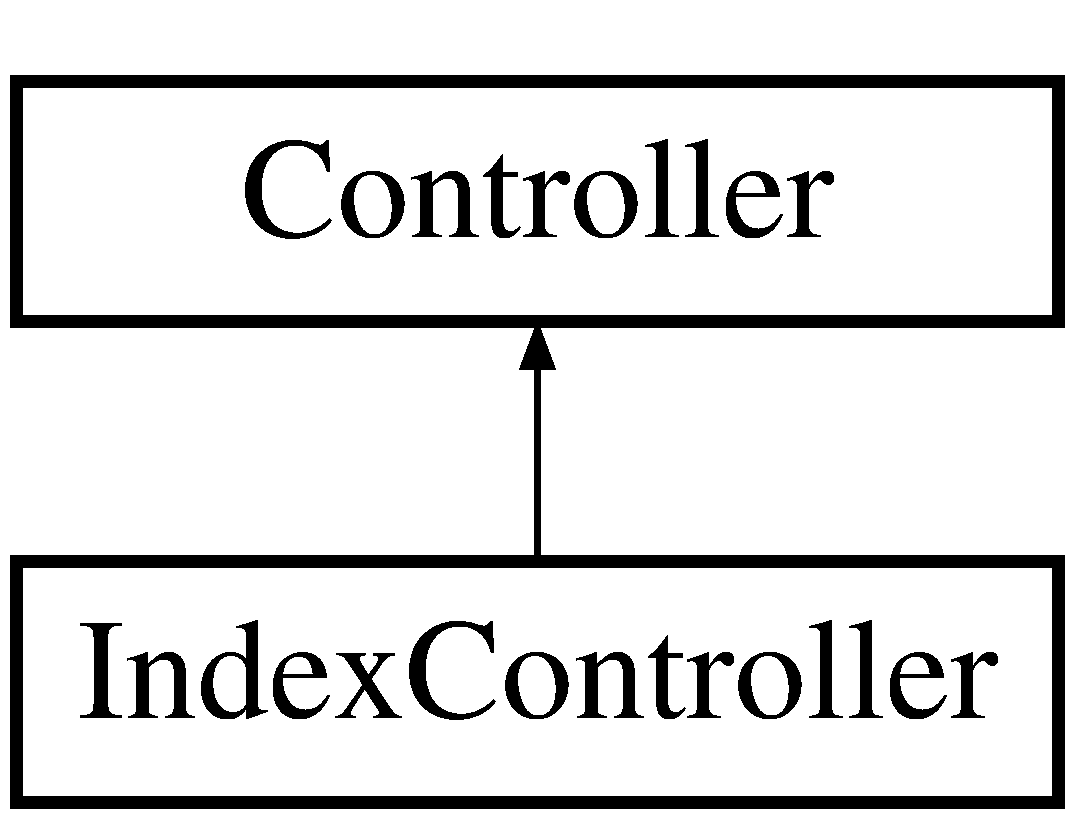
\includegraphics[height=2.000000cm]{class_index_controller}
\end{center}
\end{figure}
\subsection*{Public Member Functions}
\begin{DoxyCompactItemize}
\item 
\hypertarget{class_index_controller_a04f2101fe1cdc785b61219c2df753024}{{\bfseries index\-Action} ()}\label{class_index_controller_a04f2101fe1cdc785b61219c2df753024}

\item 
\hypertarget{class_index_controller_aa6095cbe57e0f33ed2817e90fb9c15b5}{{\bfseries snmp\-Data\-Action} (\$account\-\_\-id=null, \$tpl=null)}\label{class_index_controller_aa6095cbe57e0f33ed2817e90fb9c15b5}

\item 
\hypertarget{class_index_controller_a78f0f6573202e47da201da8ec65b47e6}{{\bfseries history\-Action} (\$account\-\_\-id=N\-U\-L\-L, \$tpl=null)}\label{class_index_controller_a78f0f6573202e47da201da8ec65b47e6}

\item 
\hypertarget{class_index_controller_a08d981933bfad63d4079e102a6c8c62e}{{\bfseries history\-Select\-Action} ()}\label{class_index_controller_a08d981933bfad63d4079e102a6c8c62e}

\item 
\hypertarget{class_index_controller_aeb878b884fc09ac18de62804e948e975}{{\bfseries error\-User\-Action} ()}\label{class_index_controller_aeb878b884fc09ac18de62804e948e975}

\end{DoxyCompactItemize}
\subsection*{Static Public Member Functions}
\begin{DoxyCompactItemize}
\item 
\hypertarget{class_index_controller_ab012c36512fb8f752dc919c64fb34648}{static {\bfseries rewrite\-\_\-file} (\$file\-\_\-path, \$mode, \$date)}\label{class_index_controller_ab012c36512fb8f752dc919c64fb34648}

\item 
\hypertarget{class_index_controller_a6d61d9eb88e39e2836595360d509c4f3}{static {\bfseries error\-Action} (Exception \$e)}\label{class_index_controller_a6d61d9eb88e39e2836595360d509c4f3}

\end{DoxyCompactItemize}
\subsection*{Data Fields}
\begin{DoxyCompactItemize}
\item 
\hypertarget{class_index_controller_a7c3eb7a98818df12bc88e63ac7ea9c63}{{\bfseries \$account\-\_\-id}}\label{class_index_controller_a7c3eb7a98818df12bc88e63ac7ea9c63}

\end{DoxyCompactItemize}
\subsection*{Additional Inherited Members}


The documentation for this class was generated from the following file\-:\begin{DoxyCompactItemize}
\item 
Controller/Index\-Controller.\-php\end{DoxyCompactItemize}

\hypertarget{class_index_model}{\section{Класс Index\-Model}
\label{class_index_model}\index{Index\-Model@{Index\-Model}}
}
\subsection*{Открытые члены}
\begin{DoxyCompactItemize}
\item 
\hyperlink{class_index_model_a5cdd544cd52782642a0f42334acdb531}{snmp\-Data} (\$account\-\_\-id, \$key, \$variable=null, \$switch\-\_\-id=null, \$port\-\_\-id=null)
\item 
\hyperlink{class_index_model_a395d66b37a253bab5365dbee626e7dbd}{get\-All\-Mac} (\$account\-\_\-id, \$pattern\-\_\-id, array \$port\-\_\-coefficient, \$switch\-\_\-id=null, \$port\-\_\-id=null)
\item 
\hyperlink{class_index_model_a92cfbe87f525727795f818072f74bb16}{cable\-Test} (\$account\-\_\-id, \$pattern\-\_\-id, \$port, \$switch\-\_\-manufacturer, \$style\-\_\-class=null, \$switch\-\_\-id=null)
\item 
\hyperlink{class_index_model_a1fce7d860847195080702dd2174e198c}{get\-Community} ()
\item 
\hyperlink{class_index_model_a99d3df1e9eea9f8bbe8be04067299e1c}{index\-Page} (\$id)
\item 
\hyperlink{class_index_model_afcec9844f30bbb9cdaf48fac789e1d7b}{snmp\-By\-Key} (\$account\-\_\-id, \$key, \$switch\-\_\-id=null, \$port\-\_\-id=null)
\item 
\hyperlink{class_index_model_ad90f0c96df11bdd429c62fa31cf226e3}{user\-Id\-By\-Port} (\$port, \$switch\-\_\-id)
\item 
\hyperlink{class_index_model_ae8029f54b6dbca39a2c9c8c80e5d24d1}{get\-Port\-Coefficient} (\$account\-\_\-id, \$port\-\_\-number, \$switch\-\_\-id)
\item 
\hyperlink{class_index_model_ad0fb7f4d93efd7678f7136d32990ee6f}{get\-User\-By\-Mac} (\$mac)
\end{DoxyCompactItemize}
\subsection*{Открытые статические члены}
\begin{DoxyCompactItemize}
\item 
static \hyperlink{class_index_model_ab17dd49d3409d5f198dffea22b33bce2}{get\-Port\-Coeff} ()
\end{DoxyCompactItemize}


\subsection{Подробное описание}


См. определение в файле Index\-Model.\-php строка 4



\subsection{Методы}
\hypertarget{class_index_model_a92cfbe87f525727795f818072f74bb16}{\index{Index\-Model@{Index\-Model}!cable\-Test@{cable\-Test}}
\index{cable\-Test@{cable\-Test}!IndexModel@{Index\-Model}}
\subsubsection[{cable\-Test}]{\setlength{\rightskip}{0pt plus 5cm}cable\-Test (
\begin{DoxyParamCaption}
\item[{}]{\$account\-\_\-id, }
\item[{}]{\$pattern\-\_\-id, }
\item[{}]{\$port, }
\item[{}]{\$switch\-\_\-manufacturer, }
\item[{}]{\$style\-\_\-class = {\ttfamily null}, }
\item[{}]{\$switch\-\_\-id = {\ttfamily null}}
\end{DoxyParamCaption}
)}}\label{class_index_model_a92cfbe87f525727795f818072f74bb16}


См. определение в файле Index\-Model.\-php строка 291

\hypertarget{class_index_model_a395d66b37a253bab5365dbee626e7dbd}{\index{Index\-Model@{Index\-Model}!get\-All\-Mac@{get\-All\-Mac}}
\index{get\-All\-Mac@{get\-All\-Mac}!IndexModel@{Index\-Model}}
\subsubsection[{get\-All\-Mac}]{\setlength{\rightskip}{0pt plus 5cm}get\-All\-Mac (
\begin{DoxyParamCaption}
\item[{}]{\$account\-\_\-id, }
\item[{}]{\$pattern\-\_\-id, }
\item[{array}]{\$port\-\_\-coefficient, }
\item[{}]{\$switch\-\_\-id = {\ttfamily null}, }
\item[{}]{\$port\-\_\-id = {\ttfamily null}}
\end{DoxyParamCaption}
)}}\label{class_index_model_a395d66b37a253bab5365dbee626e7dbd}


См. определение в файле Index\-Model.\-php строка 271

\hypertarget{class_index_model_a1fce7d860847195080702dd2174e198c}{\index{Index\-Model@{Index\-Model}!get\-Community@{get\-Community}}
\index{get\-Community@{get\-Community}!IndexModel@{Index\-Model}}
\subsubsection[{get\-Community}]{\setlength{\rightskip}{0pt plus 5cm}get\-Community (
\begin{DoxyParamCaption}
{}
\end{DoxyParamCaption}
)}}\label{class_index_model_a1fce7d860847195080702dd2174e198c}


См. определение в файле Index\-Model.\-php строка 319

\hypertarget{class_index_model_ab17dd49d3409d5f198dffea22b33bce2}{\index{Index\-Model@{Index\-Model}!get\-Port\-Coeff@{get\-Port\-Coeff}}
\index{get\-Port\-Coeff@{get\-Port\-Coeff}!IndexModel@{Index\-Model}}
\subsubsection[{get\-Port\-Coeff}]{\setlength{\rightskip}{0pt plus 5cm}static get\-Port\-Coeff (
\begin{DoxyParamCaption}
{}
\end{DoxyParamCaption}
)\hspace{0.3cm}{\ttfamily [static]}}}\label{class_index_model_ab17dd49d3409d5f198dffea22b33bce2}
\begin{DoxyReturn}{Возвращает}
array 
\end{DoxyReturn}


См. определение в файле Index\-Model.\-php строка 438

\hypertarget{class_index_model_ae8029f54b6dbca39a2c9c8c80e5d24d1}{\index{Index\-Model@{Index\-Model}!get\-Port\-Coefficient@{get\-Port\-Coefficient}}
\index{get\-Port\-Coefficient@{get\-Port\-Coefficient}!IndexModel@{Index\-Model}}
\subsubsection[{get\-Port\-Coefficient}]{\setlength{\rightskip}{0pt plus 5cm}get\-Port\-Coefficient (
\begin{DoxyParamCaption}
\item[{}]{\$account\-\_\-id, }
\item[{}]{\$port\-\_\-number, }
\item[{}]{\$switch\-\_\-id}
\end{DoxyParamCaption}
)}}\label{class_index_model_ae8029f54b6dbca39a2c9c8c80e5d24d1}


См. определение в файле Index\-Model.\-php строка 381

\hypertarget{class_index_model_ad0fb7f4d93efd7678f7136d32990ee6f}{\index{Index\-Model@{Index\-Model}!get\-User\-By\-Mac@{get\-User\-By\-Mac}}
\index{get\-User\-By\-Mac@{get\-User\-By\-Mac}!IndexModel@{Index\-Model}}
\subsubsection[{get\-User\-By\-Mac}]{\setlength{\rightskip}{0pt plus 5cm}get\-User\-By\-Mac (
\begin{DoxyParamCaption}
\item[{}]{\$mac}
\end{DoxyParamCaption}
)}}\label{class_index_model_ad0fb7f4d93efd7678f7136d32990ee6f}


См. определение в файле Index\-Model.\-php строка 422

\hypertarget{class_index_model_a99d3df1e9eea9f8bbe8be04067299e1c}{\index{Index\-Model@{Index\-Model}!index\-Page@{index\-Page}}
\index{index\-Page@{index\-Page}!IndexModel@{Index\-Model}}
\subsubsection[{index\-Page}]{\setlength{\rightskip}{0pt plus 5cm}index\-Page (
\begin{DoxyParamCaption}
\item[{}]{\$id}
\end{DoxyParamCaption}
)}}\label{class_index_model_a99d3df1e9eea9f8bbe8be04067299e1c}


См. определение в файле Index\-Model.\-php строка 343

\hypertarget{class_index_model_afcec9844f30bbb9cdaf48fac789e1d7b}{\index{Index\-Model@{Index\-Model}!snmp\-By\-Key@{snmp\-By\-Key}}
\index{snmp\-By\-Key@{snmp\-By\-Key}!IndexModel@{Index\-Model}}
\subsubsection[{snmp\-By\-Key}]{\setlength{\rightskip}{0pt plus 5cm}snmp\-By\-Key (
\begin{DoxyParamCaption}
\item[{}]{\$account\-\_\-id, }
\item[{}]{\$key, }
\item[{}]{\$switch\-\_\-id = {\ttfamily null}, }
\item[{}]{\$port\-\_\-id = {\ttfamily null}}
\end{DoxyParamCaption}
)}}\label{class_index_model_afcec9844f30bbb9cdaf48fac789e1d7b}


См. определение в файле Index\-Model.\-php строка 355

\hypertarget{class_index_model_a5cdd544cd52782642a0f42334acdb531}{\index{Index\-Model@{Index\-Model}!snmp\-Data@{snmp\-Data}}
\index{snmp\-Data@{snmp\-Data}!IndexModel@{Index\-Model}}
\subsubsection[{snmp\-Data}]{\setlength{\rightskip}{0pt plus 5cm}snmp\-Data (
\begin{DoxyParamCaption}
\item[{}]{\$account\-\_\-id, }
\item[{}]{\$key, }
\item[{}]{\$variable = {\ttfamily null}, }
\item[{}]{\$switch\-\_\-id = {\ttfamily null}, }
\item[{}]{\$port\-\_\-id = {\ttfamily null}}
\end{DoxyParamCaption}
)}}\label{class_index_model_a5cdd544cd52782642a0f42334acdb531}


См. определение в файле Index\-Model.\-php строка 82

\hypertarget{class_index_model_ad90f0c96df11bdd429c62fa31cf226e3}{\index{Index\-Model@{Index\-Model}!user\-Id\-By\-Port@{user\-Id\-By\-Port}}
\index{user\-Id\-By\-Port@{user\-Id\-By\-Port}!IndexModel@{Index\-Model}}
\subsubsection[{user\-Id\-By\-Port}]{\setlength{\rightskip}{0pt plus 5cm}user\-Id\-By\-Port (
\begin{DoxyParamCaption}
\item[{}]{\$port, }
\item[{}]{\$switch\-\_\-id}
\end{DoxyParamCaption}
)}}\label{class_index_model_ad90f0c96df11bdd429c62fa31cf226e3}


См. определение в файле Index\-Model.\-php строка 366



Объявления и описания членов класса находятся в файле\-:\begin{DoxyCompactItemize}
\item 
/home/artem/public\-\_\-html/test01/\-Model/\hyperlink{_index_model_8php}{Index\-Model.\-php}\end{DoxyCompactItemize}

\hypertarget{class_node_controller}{\section{Класс Node\-Controller}
\label{class_node_controller}\index{Node\-Controller@{Node\-Controller}}
}


Class \hyperlink{class_node_controller}{Node\-Controller}.  


Граф наследования\-:Node\-Controller\-:\begin{figure}[H]
\begin{center}
\leavevmode
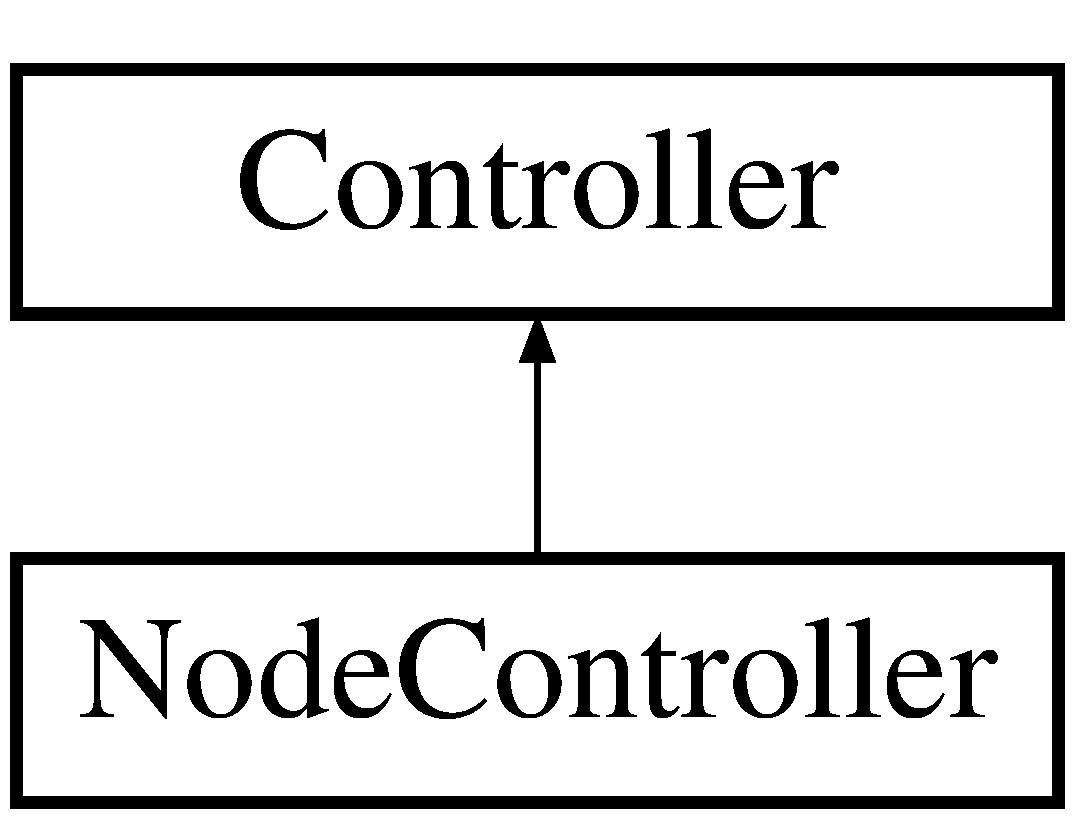
\includegraphics[height=2.000000cm]{class_node_controller}
\end{center}
\end{figure}
\subsection*{Открытые члены}
\begin{DoxyCompactItemize}
\item 
\hyperlink{class_node_controller_a04f2101fe1cdc785b61219c2df753024}{index\-Action} ()
\begin{DoxyCompactList}\small\item\em Action отвечате за загрузку обычных страниц(включая стандартных страниц ошибок) \end{DoxyCompactList}\end{DoxyCompactItemize}
\subsection*{Открытые статические члены}
\begin{DoxyCompactItemize}
\item 
static \hyperlink{class_node_controller_a2d13f67877bc056bc6798b3d0931c4a2}{write\-Error\-Data} (Exception \$e)
\begin{DoxyCompactList}\small\item\em Обработка информации выброшенных исключений \end{DoxyCompactList}\end{DoxyCompactItemize}
\subsection*{Дополнительные унаследованные члены}


\subsection{Подробное описание}
Class \hyperlink{class_node_controller}{Node\-Controller}. 

Class \hyperlink{class_node_controller}{Node\-Controller} отвечает за загрузку страниц приложения. Включает метод для загрузки стандартных страниц и страниц ошибок. Также write\-Error\-Data записывает на страницах ошибок информацию полученную из выброшенных исключений. 

См. определение в файле Node\-Controller.\-php строка 9



\subsection{Методы}
\hypertarget{class_node_controller_a04f2101fe1cdc785b61219c2df753024}{\index{Node\-Controller@{Node\-Controller}!index\-Action@{index\-Action}}
\index{index\-Action@{index\-Action}!NodeController@{Node\-Controller}}
\subsubsection[{index\-Action}]{\setlength{\rightskip}{0pt plus 5cm}index\-Action (
\begin{DoxyParamCaption}
{}
\end{DoxyParamCaption}
)}}\label{class_node_controller_a04f2101fe1cdc785b61219c2df753024}


Action отвечате за загрузку обычных страниц(включая стандартных страниц ошибок) 

Action отвечате за загрузку обычных страниц(включая стандартных страниц ошибок). Данные о необходимой странице передает объект класса \hyperlink{class_node_model}{Node\-Model}, id нужной страници получает роутер (\hyperlink{class_router}{Router}) при парсинге url. \$args массив содержит контент страници полученный \hyperlink{class_node_model}{Node\-Model} моделью из базы данных а также данные о выброшенном исключении. Передается аргументом в возвращаемую функцию рендеринга \$this-\/$>$render(\$args) \begin{DoxyReturn}{Возвращает}
\$this-\/$>$render(\$args) Функция рендеринга страници с параметром \$args 
\end{DoxyReturn}


См. определение в файле Node\-Controller.\-php строка 39

\hypertarget{class_node_controller_a2d13f67877bc056bc6798b3d0931c4a2}{\index{Node\-Controller@{Node\-Controller}!write\-Error\-Data@{write\-Error\-Data}}
\index{write\-Error\-Data@{write\-Error\-Data}!NodeController@{Node\-Controller}}
\subsubsection[{write\-Error\-Data}]{\setlength{\rightskip}{0pt plus 5cm}static write\-Error\-Data (
\begin{DoxyParamCaption}
\item[{Exception}]{\$e}
\end{DoxyParamCaption}
)\hspace{0.3cm}{\ttfamily [static]}}}\label{class_node_controller_a2d13f67877bc056bc6798b3d0931c4a2}


Обработка информации выброшенных исключений 


\begin{DoxyParams}[1]{Аргументы}
Exception & {\em \$e} & объект выброшенного исключения\\
\hline
\end{DoxyParams}
Записывает в свойства класса код ошибки и сообщение полученное из объекта \$e выброшенного исключения 

См. определение в файле Node\-Controller.\-php строка 23



Объявления и описания членов класса находятся в файле\-:\begin{DoxyCompactItemize}
\item 
/home/artem/public\-\_\-html/test01/\-Controller/\hyperlink{_node_controller_8php}{Node\-Controller.\-php}\end{DoxyCompactItemize}

\hypertarget{class_node_model}{\section{Node\-Model Class Reference}
\label{class_node_model}\index{Node\-Model@{Node\-Model}}
}
\subsection*{Public Member Functions}
\begin{DoxyCompactItemize}
\item 
\hypertarget{class_node_model_a99d3df1e9eea9f8bbe8be04067299e1c}{{\bfseries index\-Page} (\$id)}\label{class_node_model_a99d3df1e9eea9f8bbe8be04067299e1c}

\end{DoxyCompactItemize}


The documentation for this class was generated from the following file\-:\begin{DoxyCompactItemize}
\item 
Model/Node\-Model.\-php\end{DoxyCompactItemize}

\hypertarget{classpattern_model}{\section{pattern\-Model Class Reference}
\label{classpattern_model}\index{pattern\-Model@{pattern\-Model}}
}
\subsection*{Public Member Functions}
\begin{DoxyCompactItemize}
\item 
\hypertarget{classpattern_model_ae207f7fe29d94a4271fb32a156b4ce64}{{\bfseries \-\_\-\-\_\-construct} (\$account\-\_\-id)}\label{classpattern_model_ae207f7fe29d94a4271fb32a156b4ce64}

\item 
\hypertarget{classpattern_model_a4f92dd070690a6c938d15a9363065351}{{\bfseries switch\-Data} ()}\label{classpattern_model_a4f92dd070690a6c938d15a9363065351}

\item 
\hypertarget{classpattern_model_a12a4b27a766b5c4573d24e255d1ef5a4}{{\bfseries get\-Pattern\-User\-Data} ()}\label{classpattern_model_a12a4b27a766b5c4573d24e255d1ef5a4}

\item 
\hypertarget{classpattern_model_a5c106765af75e3a68d2191cdc2d784f3}{{\bfseries Pattern\-Data} (\$port\-\_\-number, \$pattern\-\_\-id)}\label{classpattern_model_a5c106765af75e3a68d2191cdc2d784f3}

\item 
\hypertarget{classpattern_model_a31f25239e28e31eb5baa5ab4564675b8}{{\bfseries mac\-Data} (\$pattern\-\_\-id)}\label{classpattern_model_a31f25239e28e31eb5baa5ab4564675b8}

\item 
\hypertarget{classpattern_model_a0f19e4f669687aaa80334bd503890fa7}{{\bfseries get\-Port\-Coefficient} (\$pattern\-\_\-id)}\label{classpattern_model_a0f19e4f669687aaa80334bd503890fa7}

\end{DoxyCompactItemize}
\subsection*{Data Fields}
\begin{DoxyCompactItemize}
\item 
\hypertarget{classpattern_model_a7c3eb7a98818df12bc88e63ac7ea9c63}{{\bfseries \$account\-\_\-id}}\label{classpattern_model_a7c3eb7a98818df12bc88e63ac7ea9c63}

\end{DoxyCompactItemize}


The documentation for this class was generated from the following file\-:\begin{DoxyCompactItemize}
\item 
Model/pattern\-Model.\-php\end{DoxyCompactItemize}

\hypertarget{class_request}{\section{Класс Request}
\label{class_request}\index{Request@{Request}}
}
\subsection*{Открытые члены}
\begin{DoxyCompactItemize}
\item 
\hyperlink{class_request_a095c5d389db211932136b53f25f39685}{\-\_\-\-\_\-construct} ()
\item 
\hyperlink{class_request_a24a9bf83a1002d46ece83a93d14bd921}{get} (\$key)
\item 
\hyperlink{class_request_a00ba439ffbc7a78df5f313ad780503d2}{post} (\$key)
\item 
\hyperlink{class_request_a53b35eef049be6f323fd8066b37d6be6}{server} (\$key)
\item 
\hyperlink{class_request_a938a7fa5c2633579704b0f4a3ded2d01}{files} (\$key)
\item 
\hyperlink{class_request_a2d62038e063e771c2fd920155f344d58}{is\-Post} ()
\end{DoxyCompactItemize}


\subsection{Подробное описание}


См. определение в файле Request.\-php строка 4



\subsection{Конструктор(ы)}
\hypertarget{class_request_a095c5d389db211932136b53f25f39685}{\index{Request@{Request}!\-\_\-\-\_\-construct@{\-\_\-\-\_\-construct}}
\index{\-\_\-\-\_\-construct@{\-\_\-\-\_\-construct}!Request@{Request}}
\subsubsection[{\-\_\-\-\_\-construct}]{\setlength{\rightskip}{0pt plus 5cm}\-\_\-\-\_\-construct (
\begin{DoxyParamCaption}
{}
\end{DoxyParamCaption}
)}}\label{class_request_a095c5d389db211932136b53f25f39685}


См. определение в файле Request.\-php строка 19



\subsection{Методы}
\hypertarget{class_request_a938a7fa5c2633579704b0f4a3ded2d01}{\index{Request@{Request}!files@{files}}
\index{files@{files}!Request@{Request}}
\subsubsection[{files}]{\setlength{\rightskip}{0pt plus 5cm}files (
\begin{DoxyParamCaption}
\item[{}]{\$key}
\end{DoxyParamCaption}
)}}\label{class_request_a938a7fa5c2633579704b0f4a3ded2d01}


См. определение в файле Request.\-php строка 44

\hypertarget{class_request_a24a9bf83a1002d46ece83a93d14bd921}{\index{Request@{Request}!get@{get}}
\index{get@{get}!Request@{Request}}
\subsubsection[{get}]{\setlength{\rightskip}{0pt plus 5cm}get (
\begin{DoxyParamCaption}
\item[{}]{\$key}
\end{DoxyParamCaption}
)}}\label{class_request_a24a9bf83a1002d46ece83a93d14bd921}


См. определение в файле Request.\-php строка 28

\hypertarget{class_request_a2d62038e063e771c2fd920155f344d58}{\index{Request@{Request}!is\-Post@{is\-Post}}
\index{is\-Post@{is\-Post}!Request@{Request}}
\subsubsection[{is\-Post}]{\setlength{\rightskip}{0pt plus 5cm}is\-Post (
\begin{DoxyParamCaption}
{}
\end{DoxyParamCaption}
)}}\label{class_request_a2d62038e063e771c2fd920155f344d58}


См. определение в файле Request.\-php строка 52

\hypertarget{class_request_a00ba439ffbc7a78df5f313ad780503d2}{\index{Request@{Request}!post@{post}}
\index{post@{post}!Request@{Request}}
\subsubsection[{post}]{\setlength{\rightskip}{0pt plus 5cm}post (
\begin{DoxyParamCaption}
\item[{}]{\$key}
\end{DoxyParamCaption}
)}}\label{class_request_a00ba439ffbc7a78df5f313ad780503d2}


См. определение в файле Request.\-php строка 33

\hypertarget{class_request_a53b35eef049be6f323fd8066b37d6be6}{\index{Request@{Request}!server@{server}}
\index{server@{server}!Request@{Request}}
\subsubsection[{server}]{\setlength{\rightskip}{0pt plus 5cm}server (
\begin{DoxyParamCaption}
\item[{}]{\$key}
\end{DoxyParamCaption}
)}}\label{class_request_a53b35eef049be6f323fd8066b37d6be6}


См. определение в файле Request.\-php строка 39



Объявления и описания членов класса находятся в файле\-:\begin{DoxyCompactItemize}
\item 
/home/artem/public\-\_\-html/test01/\-Library/\hyperlink{_request_8php}{Request.\-php}\end{DoxyCompactItemize}

\hypertarget{class_router}{\section{Router Class Reference}
\label{class_router}\index{Router@{Router}}
}
\subsection*{Static Public Member Functions}
\begin{DoxyCompactItemize}
\item 
static \hyperlink{class_router_ad6b0d5b03226bb27efd8c410c89ef635}{parse} (\$url)
\item 
\hypertarget{class_router_a7e384b5b08035be60df7696428c6cf56}{static {\bfseries get\-\_\-content\-\_\-by\-\_\-url} (\$url)}\label{class_router_a7e384b5b08035be60df7696428c6cf56}

\item 
static \hyperlink{class_router_a45e9b6bbc2e0abd383bf9a788db25dab}{get\-Url} (\$route\-Name, array \$params=array())
\item 
static \hyperlink{class_router_a0c5216068060ca9253dbad31e5895a2b}{get\-Controller} ()
\item 
static \hyperlink{class_router_af8b331d3ac442a1071aa9f7db3b60637}{get\-Action} ()
\item 
\hypertarget{class_router_a0613d1215434e1b563a42dfcd05aad60}{static {\bfseries get\-Account\-Id} ()}\label{class_router_a0613d1215434e1b563a42dfcd05aad60}

\item 
\hypertarget{class_router_acfaa3a96d0cb5a4c0d4d710dcba41e9e}{static {\bfseries get\-Id} ()}\label{class_router_acfaa3a96d0cb5a4c0d4d710dcba41e9e}

\end{DoxyCompactItemize}


\subsection{Member Function Documentation}
\hypertarget{class_router_af8b331d3ac442a1071aa9f7db3b60637}{\index{Router@{Router}!get\-Action@{get\-Action}}
\index{get\-Action@{get\-Action}!Router@{Router}}
\subsubsection[{get\-Action}]{\setlength{\rightskip}{0pt plus 5cm}static get\-Action (
\begin{DoxyParamCaption}
{}
\end{DoxyParamCaption}
)\hspace{0.3cm}{\ttfamily [static]}}}\label{class_router_af8b331d3ac442a1071aa9f7db3b60637}
\begin{DoxyReturn}{Returns}
mixed 
\end{DoxyReturn}
\hypertarget{class_router_a0c5216068060ca9253dbad31e5895a2b}{\index{Router@{Router}!get\-Controller@{get\-Controller}}
\index{get\-Controller@{get\-Controller}!Router@{Router}}
\subsubsection[{get\-Controller}]{\setlength{\rightskip}{0pt plus 5cm}static get\-Controller (
\begin{DoxyParamCaption}
{}
\end{DoxyParamCaption}
)\hspace{0.3cm}{\ttfamily [static]}}}\label{class_router_a0c5216068060ca9253dbad31e5895a2b}
\begin{DoxyReturn}{Returns}
mixed 
\end{DoxyReturn}
\hypertarget{class_router_a45e9b6bbc2e0abd383bf9a788db25dab}{\index{Router@{Router}!get\-Url@{get\-Url}}
\index{get\-Url@{get\-Url}!Router@{Router}}
\subsubsection[{get\-Url}]{\setlength{\rightskip}{0pt plus 5cm}static get\-Url (
\begin{DoxyParamCaption}
\item[{}]{\$route\-Name, }
\item[{array}]{\$params = {\ttfamily array()}}
\end{DoxyParamCaption}
)\hspace{0.3cm}{\ttfamily [static]}}}\label{class_router_a45e9b6bbc2e0abd383bf9a788db25dab}

\begin{DoxyParams}[1]{Parameters}
 & {\em \$route\-Name} & \\
\hline
array & {\em \$params} & \\
\hline
\end{DoxyParams}
\hypertarget{class_router_ad6b0d5b03226bb27efd8c410c89ef635}{\index{Router@{Router}!parse@{parse}}
\index{parse@{parse}!Router@{Router}}
\subsubsection[{parse}]{\setlength{\rightskip}{0pt plus 5cm}static parse (
\begin{DoxyParamCaption}
\item[{}]{\$url}
\end{DoxyParamCaption}
)\hspace{0.3cm}{\ttfamily [static]}}}\label{class_router_ad6b0d5b03226bb27efd8c410c89ef635}

\begin{DoxyParams}{Parameters}
{\em \$url} & \\
\hline
\end{DoxyParams}

\begin{DoxyExceptions}{Exceptions}
{\em Exception} & \\
\hline
\end{DoxyExceptions}


The documentation for this class was generated from the following file\-:\begin{DoxyCompactItemize}
\item 
Library/Router.\-php\end{DoxyCompactItemize}

\hypertarget{class_session}{\section{Класс Session}
\label{class_session}\index{Session@{Session}}
}
\subsection*{Открытые статические члены}
\begin{DoxyCompactItemize}
\item 
static \hyperlink{class_session_a8f660283f72e0f3c5f00b4f98563a79b}{has} (\$key)
\item 
static \hyperlink{class_session_a4ecf4c33104949ba1a007a73d71dbb15}{set} (\$key, \$val)
\item 
static \hyperlink{class_session_a292b7d28cfcd001085631b11754a3a67}{has\-User} (\$user\-\_\-name)
\item 
static \hyperlink{class_session_a15e2679f2a8f6fa4d60757f4d65413ac}{get} (\$key)
\item 
static \hyperlink{class_session_acc60f64095c2df2c0d1e48f9f3ffb9d8}{remove} (\$key)
\item 
static \hyperlink{class_session_a146085d0f3a9d17bdcd7f3d4081d8c0d}{start} ()
\item 
static \hyperlink{class_session_a93d4348dfe017e3b97a7131f03897121}{destroy} ()
\item 
static \hyperlink{class_session_aa7c4da247e52be9a1eb10db617faba68}{set\-Flash} (\$message, \$warning\-\_\-class=null)
\item 
static \hyperlink{class_session_ae4c4b98671bdd1fbfe4ae9defb5405ad}{get\-Flash} (\$account\-\_\-id=null, \$switch\-\_\-id=null, \$port\-\_\-id=null, \$switch\-\_\-port\-\_\-id=null)
\end{DoxyCompactItemize}
\subsection*{Статические открытые данные}
\begin{DoxyCompactItemize}
\item 
static \hyperlink{class_session_a5bacf7bbae287dfd28fbaad90f463720}{\$flash\-\_\-messages} = array()
\end{DoxyCompactItemize}


\subsection{Подробное описание}


См. определение в файле Session.\-php строка 4



\subsection{Методы}
\hypertarget{class_session_a93d4348dfe017e3b97a7131f03897121}{\index{Session@{Session}!destroy@{destroy}}
\index{destroy@{destroy}!Session@{Session}}
\subsubsection[{destroy}]{\setlength{\rightskip}{0pt plus 5cm}static destroy (
\begin{DoxyParamCaption}
{}
\end{DoxyParamCaption}
)\hspace{0.3cm}{\ttfamily [static]}}}\label{class_session_a93d4348dfe017e3b97a7131f03897121}


См. определение в файле Session.\-php строка 48

\hypertarget{class_session_a15e2679f2a8f6fa4d60757f4d65413ac}{\index{Session@{Session}!get@{get}}
\index{get@{get}!Session@{Session}}
\subsubsection[{get}]{\setlength{\rightskip}{0pt plus 5cm}static get (
\begin{DoxyParamCaption}
\item[{}]{\$key}
\end{DoxyParamCaption}
)\hspace{0.3cm}{\ttfamily [static]}}}\label{class_session_a15e2679f2a8f6fa4d60757f4d65413ac}


См. определение в файле Session.\-php строка 28

\hypertarget{class_session_ae4c4b98671bdd1fbfe4ae9defb5405ad}{\index{Session@{Session}!get\-Flash@{get\-Flash}}
\index{get\-Flash@{get\-Flash}!Session@{Session}}
\subsubsection[{get\-Flash}]{\setlength{\rightskip}{0pt plus 5cm}static get\-Flash (
\begin{DoxyParamCaption}
\item[{}]{\$account\-\_\-id = {\ttfamily null}, }
\item[{}]{\$switch\-\_\-id = {\ttfamily null}, }
\item[{}]{\$port\-\_\-id = {\ttfamily null}, }
\item[{}]{\$switch\-\_\-port\-\_\-id = {\ttfamily null}}
\end{DoxyParamCaption}
)\hspace{0.3cm}{\ttfamily [static]}}}\label{class_session_ae4c4b98671bdd1fbfe4ae9defb5405ad}


См. определение в файле Session.\-php строка 74

\hypertarget{class_session_a8f660283f72e0f3c5f00b4f98563a79b}{\index{Session@{Session}!has@{has}}
\index{has@{has}!Session@{Session}}
\subsubsection[{has}]{\setlength{\rightskip}{0pt plus 5cm}static has (
\begin{DoxyParamCaption}
\item[{}]{\$key}
\end{DoxyParamCaption}
)\hspace{0.3cm}{\ttfamily [static]}}}\label{class_session_a8f660283f72e0f3c5f00b4f98563a79b}


См. определение в файле Session.\-php строка 8

\hypertarget{class_session_a292b7d28cfcd001085631b11754a3a67}{\index{Session@{Session}!has\-User@{has\-User}}
\index{has\-User@{has\-User}!Session@{Session}}
\subsubsection[{has\-User}]{\setlength{\rightskip}{0pt plus 5cm}static has\-User (
\begin{DoxyParamCaption}
\item[{}]{\$user\-\_\-name}
\end{DoxyParamCaption}
)\hspace{0.3cm}{\ttfamily [static]}}}\label{class_session_a292b7d28cfcd001085631b11754a3a67}


См. определение в файле Session.\-php строка 20

\hypertarget{class_session_acc60f64095c2df2c0d1e48f9f3ffb9d8}{\index{Session@{Session}!remove@{remove}}
\index{remove@{remove}!Session@{Session}}
\subsubsection[{remove}]{\setlength{\rightskip}{0pt plus 5cm}static remove (
\begin{DoxyParamCaption}
\item[{}]{\$key}
\end{DoxyParamCaption}
)\hspace{0.3cm}{\ttfamily [static]}}}\label{class_session_acc60f64095c2df2c0d1e48f9f3ffb9d8}


См. определение в файле Session.\-php строка 36

\hypertarget{class_session_a4ecf4c33104949ba1a007a73d71dbb15}{\index{Session@{Session}!set@{set}}
\index{set@{set}!Session@{Session}}
\subsubsection[{set}]{\setlength{\rightskip}{0pt plus 5cm}static set (
\begin{DoxyParamCaption}
\item[{}]{\$key, }
\item[{}]{\$val}
\end{DoxyParamCaption}
)\hspace{0.3cm}{\ttfamily [static]}}}\label{class_session_a4ecf4c33104949ba1a007a73d71dbb15}


См. определение в файле Session.\-php строка 13

\hypertarget{class_session_aa7c4da247e52be9a1eb10db617faba68}{\index{Session@{Session}!set\-Flash@{set\-Flash}}
\index{set\-Flash@{set\-Flash}!Session@{Session}}
\subsubsection[{set\-Flash}]{\setlength{\rightskip}{0pt plus 5cm}static set\-Flash (
\begin{DoxyParamCaption}
\item[{}]{\$message, }
\item[{}]{\$warning\-\_\-class = {\ttfamily null}}
\end{DoxyParamCaption}
)\hspace{0.3cm}{\ttfamily [static]}}}\label{class_session_aa7c4da247e52be9a1eb10db617faba68}


См. определение в файле Session.\-php строка 53

\hypertarget{class_session_a146085d0f3a9d17bdcd7f3d4081d8c0d}{\index{Session@{Session}!start@{start}}
\index{start@{start}!Session@{Session}}
\subsubsection[{start}]{\setlength{\rightskip}{0pt plus 5cm}static start (
\begin{DoxyParamCaption}
{}
\end{DoxyParamCaption}
)\hspace{0.3cm}{\ttfamily [static]}}}\label{class_session_a146085d0f3a9d17bdcd7f3d4081d8c0d}


См. определение в файле Session.\-php строка 43



\subsection{Поля}
\hypertarget{class_session_a5bacf7bbae287dfd28fbaad90f463720}{\index{Session@{Session}!\$flash\-\_\-messages@{\$flash\-\_\-messages}}
\index{\$flash\-\_\-messages@{\$flash\-\_\-messages}!Session@{Session}}
\subsubsection[{\$flash\-\_\-messages}]{\setlength{\rightskip}{0pt plus 5cm}\$flash\-\_\-messages = array()\hspace{0.3cm}{\ttfamily [static]}}}\label{class_session_a5bacf7bbae287dfd28fbaad90f463720}


См. определение в файле Session.\-php строка 6



Объявления и описания членов класса находятся в файле\-:\begin{DoxyCompactItemize}
\item 
/home/artem/public\-\_\-html/test01/\-Library/\hyperlink{_session_8php}{Session.\-php}\end{DoxyCompactItemize}

%--- End generated contents ---

% Index
\newpage
\phantomsection
\addcontentsline{toc}{chapter}{Index}
\printindex

\end{document}
